%%%% CAPÍTULO 2 - REVISÃO DA LITERATURA (OU REVISÃO BIBLIOGRÁFICA, ESTADO DA ARTE, ESTADO DO CONHECIMENTO)
%%
%% O autor deve registrar seu conhecimento sobre a literatura básica do assunto, discutindo e comentando a informação já publicada.
%% A revisão deve ser apresentada, preferencialmente, em ordem cronológica e por blocos de assunto, procurando mostrar a evolução do tema.
%% Título e rótulo de capítulo (rótulos não devem conter caracteres especiais, acentuados ou cedilha)
\chapter{Referencial te\'orico}\label{cap:referencialTeorico}

Esta seção reúne os fundamentos teóricos que sustentam o desenvolvimento deste estudo, abordando os conceitos essenciais sobre labirintos, LLMs, estratégias de fine-tuning e métodos de explicabilidade.

\section{Labirintos e Raciocínio Espacial}

Labirintos são estruturas clássicas amplamente utilizadas para investigar processos de raciocínio espacial, planejamento e navegação, especialmente no contexto de agentes artificiais \cite{vartak2023mazesolverrobot}. Conceitualmente, um labirinto pode ser definido como um ambiente composto por caminhos interconectados, obstáculos e pontos de decisão, cujo objetivo é encontrar uma rota eficiente entre um ponto de entrada e um de saída. A resolução de labirintos demanda a construção de representações espaciais internas, identificação de padrões e adaptação de estratégias a partir da estrutura do ambiente, como \cite{sadik2010comprehensive} aborda comparando diferentes técnicas baseadas em teoria dos grafos.

Neste trabalho, labirintos em ASCII são empregados como um domínio controlado para testar a capacidade de modelos de linguagem em desenvolver representações espaciais e estratégias de navegação a partir de entradas exclusivamente textuais. Essa escolha permite investigar, com o apoio de técnicas de explicabilidade, se os modelos são capazes de realizar raciocínio estrutural coerente ou se apenas se baseiam em padrões estatísticos superficiais.

\section{LLMs - Large Language Models}

Os LLMs representam um marco no avanço do Processamento de Linguagem Natural (PLN), resultado de uma trajetória que abrange: modelos estatísticos, como n-gram; passando por modelos baseados em \textit{word embeddings}, como Word2Vec \cite{mikolov2013distributed}; \textit{Recurrent Neural Networks} (RNNs) e \textit{Long Short-Term Memory} (LSTM) \cite{hochreiter1997long} e, mais recentemente, arquiteturas baseadas em \textit{transformers} \cite{jurafsky2025slp3}.

\subsection{Arquitetura Transformer e Mecanismo de Atenção}

O desenvolvimento dos LLMs está diretamente ligado à evolução dos transformers, introduzidos por \cite{vaswani2023transformers}, que revolucionaram o campo ao permitir a modelagem eficiente de dependências contextuais de longo alcance, por meio de mecanismos de atenção. Sua arquitetura é composta por blocos de \textit{encoder} e \textit{decoder}, que podem ser utilizados separadamente ou em conjunto, conforme a tarefa. A figura \ref{fig:transformer-architecture} ilustra a arquitetura básica de um transformer, destacando seus componentes principais.

\begin{figure}[h!]
    \centering
    \caption{Arquitetura básica de um transformer, com blocos de encoder e decoder}
    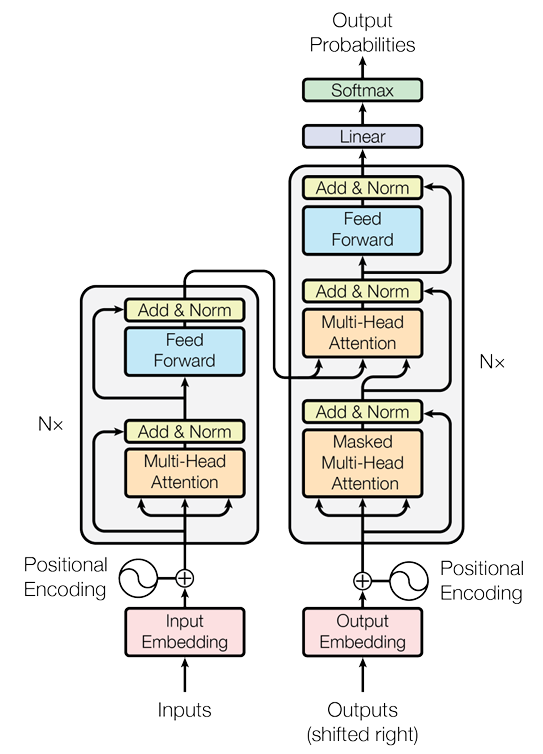
\includegraphics[width=0.5\textwidth]{./figuras/transformer-architecture.png}
    \label{fig:transformer-architecture}
    \fonte{\citet{vaswani2023transformers}}
\end{figure}

Modelos recentes, como o BERT \cite{devlin2019bert}, utilizam apenas o encoder, sendo eficazes em tarefas de compreensão textual, enquanto modelos GPT \cite{yenduri2023gpt} utilizam apenas o decoder, focando na geração de texto. Arquiteturas encoder-decoder, como o T5 \cite{raffel2023t5}, são empregadas em tarefas de tradução e sumarização \cite{tunstall2022nlptransformers}.

\section{Fine-tuning de LLMs}\label{sec:fund-finetuning}

O \textit{fine-tuning} é uma etapa fundamental para adaptar LLMs a tarefas específicas, permitindo que modelos previamente treinados em grandes volumes de dados textuais sejam ajustados para contextos e domínios particulares. Neste trabalho, destacam-se duas estratégias principais: o \textbf{Supervised Fine-Tuning (SFT)} e o \textbf{Group Relative Policy Optimization (GRPO)}.

O \textbf{SFT} consiste no ajuste supervisionado do modelo utilizando conjuntos de dados rotulados, nos quais o modelo aprende a associar instruções ou entradas a saídas desejadas. Essa técnica é amplamente empregada para especializar LLMs em tarefas como classificação, tradução e, no contexto deste estudo, navegação em labirintos ASCII. O processo envolve a construção de um dataset de pares (instrução, saída) e o treinamento supervisionado para minimizar o erro entre a resposta do modelo e a resposta esperada \cite{zhang2024instructiontuning}. O SFT é considerado eficiente, pois permite adaptar rapidamente o modelo a novos domínios sem a necessidade de re-treinamento completo.

Já o \textbf{GRPO} é uma técnica baseada em otimização de políticas relativas a grupos, utilizada para aprimorar o desempenho do modelo considerando preferências coletivas de múltiplos usuários ou agentes. No GRPO, o modelo é ajustado para maximizar a satisfação de critérios definidos por grupos, promovendo respostas mais alinhadas a contextos colaborativos ou multiusuário \cite{dao2025alphamaze}. Essa abordagem é especialmente relevante em cenários onde a diversidade de preferências e estratégias é importante para o sucesso da tarefa.

Essas estratégias são relevantes para o presente estudo, pois permitem investigar como diferentes métodos de ajuste podem impactar o desempenho dos LLMs em tarefas de raciocínio espacial.

\section{Explicabilidade em LLMs}

Apesar do alto desempenho, LLMs são frequentemente criticados por seu caráter de “caixa-preta”, dificultando o entendimento sobre como tomam decisões e levantando preocupações éticas e de confiança \cite{zhao2023explainability, cambria2024xai, luo2024fromunderstanding}. A opacidade desses modelos pode resultar em respostas inesperadas, enviesadas ou até mesmo em alucinações, o que reforça a necessidade de técnicas de explicabilidade (\textit{explainability}) para tornar seus mecanismos internos mais transparentes.

A explicabilidade em LLMs pode ser abordada sob diferentes perspectivas. Do ponto de vista do usuário final, explicações claras e acessíveis são essenciais para promover confiança e permitir o uso responsável dos modelos em aplicações sensíveis, como saúde, educação e finanças. Para pesquisadores e desenvolvedores, a explicabilidade atua como ferramenta de diagnóstico, facilitando a identificação de vieses, falhas e oportunidades de aprimoramento dos modelos \cite{zhao2023explainability, luo2024fromunderstanding}.

As principais técnicas de explicabilidade para LLMs incluem métodos de atribuição de importância a tokens (feature attribution), análise de camadas internas, visualização de mecanismos de atenção e explicações baseadas em exemplos. Recentemente, abordagens baseadas em prompts e cadeias de raciocínio (\textit{chain-of-thought} \cite{wei2023chainofthought}) também têm sido exploradas para tornar o processo de decisão dos modelos mais interpretável \cite{zhao2023explainability}. No entanto, o aumento da escala e da complexidade dos LLMs impõe desafios adicionais, tornando a geração de explicações confiáveis e compreensíveis uma tarefa ainda em aberto.

Além disso, a literatura destaca a importância de desenvolver métricas e benchmarks específicos para avaliar a qualidade das explicações geradas, bem como de promover a integração entre avanços em LLMs e técnicas de XAI (Explainable AI) \cite{cambria2024xai}. O avanço conjunto dessas áreas é fundamental para garantir o uso ético, seguro e transparente dos modelos de linguagem em aplicações reais.

\subsection{LLM-MRI}

A biblioteca LLM-MRI (\textit{Large Language Model - Magnetic Resonance Imaging}) é uma ferramenta de código aberto desenvolvida para simplificar o estudo de padrões de ativação em LLMs baseados na arquitetura \textit{transformer}. Atuando de forma análoga a uma ressonância magnética em cérebros biológicos, a ferramenta permite mapear e visualizar regiões neurais ativas durante o processamento de textos, transformando vetores de alta dimensionalidade em representações analisáveis.

O funcionamento da biblioteca estrutura-se em três estágios sequenciais: (1) Extração de Ativações, (2) Mapeamento de Regiões Neurais e (3) Geração de Artefatos. O fluxo completo de processamento está ilustrado na Figura \ref{fig:fluxograma-llmmri}.

\begin{figure}[h!]
    \centering
    \caption{Fluxograma de funcionamento da biblioteca LLM-MRI}
    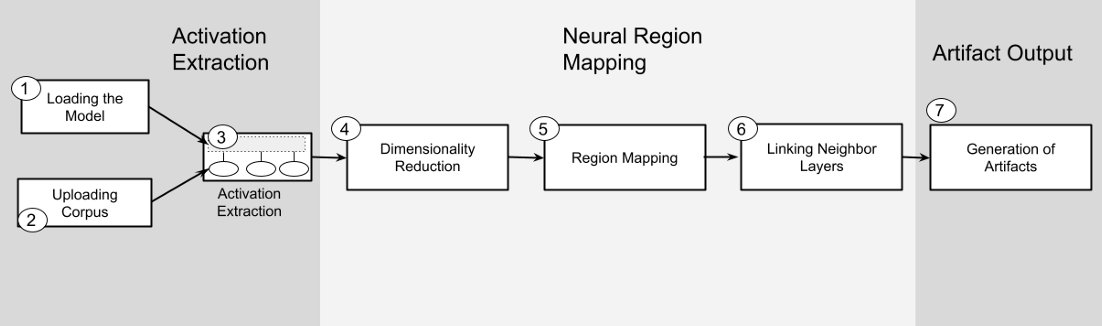
\includegraphics[width=1.0\textwidth]{figuras/fluxograma-funcionamento-llmmri.png}
    \label{fig:fluxograma-llmmri}
    \fonte{\citet{costa2024llmmri}}
\end{figure}

Na etapa inicial, denominada \textbf{Extração de Ativações} (passos 1 a 3 na \autoref{fig:fluxograma-llmmri}), o modelo e o \textit{corpus} de texto são carregados. A ferramenta foca na extração das ativações das camadas \textit{feed-forward}, partindo da premissa de que estas carregam maior significado semântico e são mais propícias ao mapeamento de áreas neurais do que os mecanismos de atenção isolados.

O segundo estágio, \textbf{Mapeamento de Regiões Neurais}, constitui o núcleo de funcionamento da ferramenta. Devido à alta dimensionalidade dos LLMs, a biblioteca aplica técnicas de redução de dimensionalidade (como UMAP) para projetar os neurônios em um espaço bidimensional (passo 4). Em seguida, este espaço é discretizado em ''regiões neurais`` (passo 5), que agregam neurônios com padrões de ativações semelhantes. A partir desse mapeamento, a ferramenta constrói um grafo (passo 6) onde:

\begin{itemize}
    \item Os \textbf{nós} representam as regiões neurais ativas;
    \item As \textbf{arestas} representam o fluxo de ativação entre camadas vizinhas, ponderadas pela frequência de coativação estimulada pelos documentos processados.
\end{itemize}

Por fim, no estágio de \textbf{Geração de Artefatos} (passo 7), a LLM-MRI produz visualizações das camadas ativas e modelos de grafos compatíveis com bibliotecas de análise de redes (como \textit{NetworkX}). Esses grafos permitem a aplicação de métricas de Redes Complexas (e.g. centralidade, densidade e clusterização) para realizar avaliações quantitativas e qualitativas da estrutura interna do modelo.

No contexto deste trabalho, a capacidade da LLM-MRI de gerar grafos interconectados das camadas internas é utilizada para investigar se o aprendizado da tarefa de navegação em labirintos provoca alterações estruturais mensuráveis na topologia das ativações dos modelos, contribuindo para a análise da interpretabilidade e do raciocínio espacial dos modelos.
